% Intended LaTeX compiler: pdflatex
\documentclass[11pt]{article}
\usepackage[utf8]{inputenc}
\usepackage[T1]{fontenc}
\usepackage{graphicx}
\usepackage{grffile}
\usepackage{longtable}
\usepackage{wrapfig}
\usepackage{rotating}
\usepackage[normalem]{ulem}
\usepackage{amsmath}
\usepackage{textcomp}
\usepackage{amssymb}
\usepackage{capt-of}
\usepackage{hyperref}
\author{Nick Anderson}
\date{\today}
\title{State of the CFEngine\\\medskip
\large Or Since last time at Config Management Camp}
\hypersetup{
 pdfauthor={Nick Anderson},
 pdftitle={State of the CFEngine},
 pdfkeywords={},
 pdfsubject={},
 pdfcreator={Emacs 25.2.2 (Org mode 9.1.6)}, 
 pdflang={English}}
\begin{document}

\maketitle

\section*{}
\label{sec:org3e38e4b}

\section*{Releases}
\label{sec:org93816a3}
5 releases since 2017-01-01


\begin{center}
\begin{tabular}{rr}
Version & Date\\
\hline
3.7.5 & 2017-03-30\\
3.10.1 & 2017-03-30\\
3.10.2 & 2017-08-11\\
3.11.0 & 2017-08-11\\
3.7.6 & 2017-09-12\\
\end{tabular}
\end{center}

\section*{Contributions}
\label{sec:org2e7d66b}
\begin{center}
\label{tab:org67eb355}
\begin{tabular}{lrrr}
 & Core & MPF & Docs\\
Commits & 256 & 163 & 207\\
Contributors & 24 & 14 & 17\\
New Contributors & 9 & 4 & 6\\
\end{tabular}
\end{center}

\section*{Core Functionality}
\label{sec:org4564deb}
\subsection*{\texttt{with} attribute}
\label{sec:orgb653bd2}

\begin{verbatim}
bundle agent main
{
  vars:
      "todo" slist => { "a 1", "b 2", "c 3" };
      # Here, `with` is the canonified version of $(todo), letting us avoid an

      # intermediate canonification array.
      "$(with)" string => "$(todo)", with => canonify($(todo));

      "complex" data => '
{
  "x": 200,
  "y": [ 1, 2, null, true, false ]
}
';

  reports:
      "For iterable '$(todo)' we created variable '$(with)' and its value is '$(todo)'"
        with => canonify($(todo));

      "We can print a data container compactly without creating a temporary variable: $(with)"
        with => format("%S", complex);

      "We can print a data container fully without creating a temporary variable: $(with)"
        with => storejson(complex);
}
\end{verbatim}
\captionof{figure}{\label{orgbcf8039}
With attribute usage example policy}

\subsection*{\texttt{with} attribute}
\label{sec:org28cd640}

\begin{verbatim}
R: For iterable 'a 1' we created variable 'a_1' and its value is 'a 1'
R: For iterable 'b 2' we created variable 'b_2' and its value is 'b 2'
R: For iterable 'c 3' we created variable 'c_3' and its value is 'c 3'
R: We can print a data container compactly without creating a temporary variable: {"x":200,"y":[1,2,null,true,false]}
R: We can print a data container fully without creating a temporary variable: {
  "x": 200,
  "y": [
    1,
    2,
    null,
    true,
    false
  ]
}
\end{verbatim}

\subsection*{\texttt{inline\_mustache}}
\label{sec:orge726f0e}

\begin{NOTES}
You are no longer required to use an external file template. Now you can
provide the template directly within the policy.
\end{NOTES}

\begin{verbatim}
bundle agent main
{
  vars:
    "d" data => '{ "hello": "world", "feature": [ "render", "inline", "mustache" ] }';

  files:

    "/tmp/example.txt"
      create => "true",
      template_method => "inline_mustache",
      edit_template_string => "{{%-top-}}",
      template_data => @(d);

}
\end{verbatim}
\captionof{figure}{Example \texttt{template\_method} \texttt{inline\_mustache}}

\subsection*{\texttt{inline\_mustache}}
\label{sec:orgb5ccdb9}

Results in \texttt{/tmp/example.txt} having this content.

\begin{verbatim}
{
  "feature": [
    "render",
    "inline",
    "mustache"
  ],
  "hello": "world"
}
\end{verbatim}
\captionof{figure}{Example \texttt{template\_method} \texttt{inline\_mustache}}
\subsection*{Multiple augments}
\label{sec:org945c492}

\textbf{NOTE:} Current implementation discussion in progress in \href{https://tracker.mender.io/browse/CFE-2741}{CFE-2741}. Please
consider participating.

\begin{verbatim}
{
  "vars":{
    "my_var": "defined in def.json",
    "my_other_var": "Defined ONLY in def.json"
  },
  "augments": [
    "/tmp/$(sys.flavor).json"
  ]
}
\end{verbatim}
\captionof{figure}{Example \texttt{/tmp/def.json}}

\subsection*{Multiple augments}
\label{sec:org052bdf0}

\begin{verbatim}
{
  "vars": {
    "my_var": "Overridden in centos_6.json",
    "centos_6_var": "Defined ONLY in centos_6.json"
  }
}
\end{verbatim}
\captionof{figure}{Example \texttt{/tmp/centos\_6.json}}

\subsection*{Multiple augments}
\label{sec:org77c0e35}

\begin{verbatim}
[root@hub tmp]# cf-agent -KIf ./example.cf 
R: def.my_var == Overridden in centos_6.json
R: def.my_other_var == Defined ONLY in def.json
R: def.centos_6_var == Defined ONLY in centos_6.json
\end{verbatim}

\subsection*{\texttt{missing\_ok}}
\label{sec:org8ee3217}
\section*{MPF Functionality}
\label{sec:orga7af1b8}
\subsection*{Augments - Append the \texttt{bundlesequnece} of \texttt{promises.cf} and \texttt{update.cf}}
\label{sec:orgb1b3403}

\begin{itemize}
\item \texttt{control\_common\_bundlesequence\_end}
\item \texttt{control\_common\_update\_bundlesequence\_end}
\end{itemize}

\begin{verbatim}
{
  "vars":{
    "control_common_bundlesequence_end": [ "mybundle1", "mybundle2" ],
    "control_common_update_bundlesequence_end": [ "my_updatebundle1", "mybundle2" ]
  }
}
\end{verbatim}

\begin{itemize}
\item Order of bundle actuation not guaranteed.
\item Agent errors if named bundle is missing.
\end{itemize}

\subsection*{Augments - Log file retention and rotation limits}
\label{sec:orgaae6216}

\begin{description}
\item[{\texttt{mpf\_log\_files\_max\_size}}] Max file size before rotation
\item[{\texttt{mpf\_log\_file\_retention}}] Number of file rotations to keep
\item[{\texttt{mpf\_log\_dir\_retention}}] Number of file rotations to keep in \texttt{outputs},
\texttt{reports}, and the Enterprise application log directory.
\end{description}

\begin{verbatim}
{
  "vars": {
    "mpf_log_file_retention": "5",
    "mpf_log_file_max_size": "10M",
    "mpf_log_dir_retention": "7"
  }
}
\end{verbatim}

\subsection*{Augments - Execution schedule}
\label{sec:org0f9b0ce}

\begin{description}
\item[{\texttt{control\_executor\_schedule}}] Classes that trigger execution of \texttt{cf-agent}.
\end{description}

\begin{verbatim}
{
  "vars": {
    "control_executor_schedule": [ "Min00", "Min30" ]
  }
}
\end{verbatim}

\subsection*{Augments - \texttt{splaytime}}
\label{sec:org77cb975}

\begin{description}
\item[{\texttt{control\_executor\_splaytime}}] Maximum number of minutes \texttt{exec\_commad} should
wait before executing.
\end{description}

\begin{verbatim}
{
  "vars": {
    "control_executor_splaytime": "3"
  }
}
\end{verbatim}

\subsection*{Augments - \texttt{allowlegacyconnects}}
\label{sec:orgd61e204}

\begin{description}
\item[{\texttt{control\_server\_allowlegacyconnects}}] List of subnets allowed to connect
using legacy protocol (versions prior to 3.7.0).
\end{description}

\begin{verbatim}
{
  "vars": {
    "control_server_allowlegacyconnects": [ "0.0.0.0/0" ]
  }
}
\end{verbatim}

\subsection*{Augments - \texttt{maxconnections}}
\label{sec:org2d82bcb}

\begin{description}
\item[{\texttt{control\_serverd\_maxconnections}}] Maximum number of connections allowed by
\texttt{cf-serverd}.
\end{description}

\begin{verbatim}
{
  "vars":{
      "control_serverd_maxconnections": "1000"
  }
}
\end{verbatim}

\subsection*{Augments - Client initiated reporting (Enterprise)}
\label{sec:org350c13d}

\begin{description}
\item[{\texttt{control\_hub\_exclude\_hosts}}] List of subnets to exclude from hub initiated
report collection.
\item[{\texttt{client\_initiated\_reporting\_enabled}}] List of classes that if defined should
initiate reporting to an enterprise hub.
\item[{\texttt{control\_server\_call\_collect\_interval}}] Number of minutes between client
initiated reporting.
\end{description}

\begin{verbatim}
{
    "vars": {
        "control_server_call_collect_interval": "1",
        "control_hub_exclude_hosts": [ "0.0.0.0/0" ]
    },

    "classes" {
        "client_initiated_reporting_enabled": [ "any" ]
    }
}
\end{verbatim}

\subsection*{Augments - \texttt{files\_single\_copy}}
\label{sec:org3910fbd}

\begin{description}
\item[{\texttt{control\_agent\_files\_single\_copy}}] List of regular expressions matching
files that should not be copied more than once.
\end{description}

\begin{verbatim}
{
  "vars":{
    "control_agent_files_single_copy": [ ".*" ]
  }

}
\end{verbatim}

\subsection*{Augments - \texttt{default\_repository}}
\label{sec:org1209b12}

\begin{description}
\item[{\texttt{mpf\_control\_agent\_default\_repository}}] List of classes class will cause
these backups to be placed in \texttt{\$(sys.workdir)/backups}.

\item[{\texttt{control\_agent\_default\_backup}}] Directory where backups should be placed
(defaults to \texttt{\$(sys.workdir/backups}).
\end{description}

\begin{verbatim}

{
  "classes": {
    "mpf_control_agent_default_repository": [ "any" ]
  },

  "vars": {
    "control_agent_default_repository": "/var/cfengine/edit_backups"
  }
}
\end{verbatim}

\subsection*{\texttt{templates} shortcut}
\label{sec:org90caa4c}

\begin{description}
\item[{\texttt{dir\_templates}}] Path to common template directory. Shortcut provided by
\texttt{cf-serverd} as \texttt{templates/}.

\begin{verbatim}
{
    "vars": {
        "dir_templates": "/var/cfengine/mytemplates"
        }
}
\end{verbatim}
\end{description}

\begin{verbatim}
bundle agent example
{
  files:

    "$(def.dir_templates)/mytemplate.mustache" -> { "myservice" }

      copy_from => remote_dcp( "templates/mytemplate.mustache",
                               $(sys.policy_server) ),

      comment => "mytemplate is necessary in order to render
                  myservice configuration file.";
}
\end{verbatim}

\subsection*{Automatically restart components on related data change}
\label{sec:org56b9bf1}

\begin{NOTES}
While the agent itsef will reload its config upon notice of policy change this
bundle specifically handles changes to variables used in the MPF which may come
from external data sources which are unknown to the components themselves.
\end{NOTES}

\begin{description}
\item[{\texttt{mpf\_augments\_control\_enabled}}] List of classes that automatic component
restart on related data change should be enabled for.
\end{description}

\begin{verbatim}
{
  "classes":{
      "mpf_augments_control_enabled": [ "any" ]
  }
}
\end{verbatim}

\subsection*{Host info report now now renders inventory variables}
\label{sec:org011b701}

\begin{verbatim}
cf-agent -KIb host_info_report
\end{verbatim}

\begin{verbatim}
### Inventory

#### Variables tagged for inventory

{
  "default:cfe_autorun_inventory_disk.free": "5.00",
  "default:cfe_autorun_inventory_listening_ports.ports": [
    "22",
    "25",
    "53",
  ],
  "default:cfe_autorun_inventory_memory.total": "32050.27",
  "default:sys.arch": "x86_64",
  "default:sys.cf_version": "3.11.0",
  "default:sys.class": "linux",
  "default:sys.cpus": "4",
  "default:sys.flavor": "ubuntu_17",
  "default:sys.hardware_addresses": [
    "5c:e0:c5:9f:f3:8f",
    "52:54:00:6b:62:06",
    "02:42:79:79:f6:02",
    "0a:00:27:00:00:00"
  ],
  "default:sys.inet": {
    "default_gateway": "192.168.42.1",
\end{verbatim}
\captionof{figure}{Sample from inventory section of host info report}

\section*{Enterprise Functionality}
\label{sec:orgfe44e59}
\subsection*{UI responsiveness}
\label{sec:org987f090}
\begin{itemize}
\item \href{data/75/971753-cddb-4739-a0a1-dcb66df44ab9/alert-status-speed-comparison.webm}{Testing} with 50,000 host data sets
\end{itemize}

\subsection*{Global Host Search}
\label{sec:org657be7b}
\begin{itemize}
\item Easily find hosts by name, ip or identity
\end{itemize}

\begin{center}
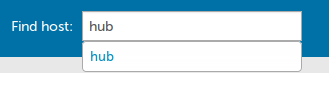
\includegraphics[width=.9\linewidth]{data/f9/7c9b4d-d46f-4aee-bd68-630f44106b0e/2018-01-14_Selection_002_2018-01-14_13-21-21.png}
\end{center}

\subsection*{host count trend widget}
\label{sec:orgc7512ff}
\begin{center}
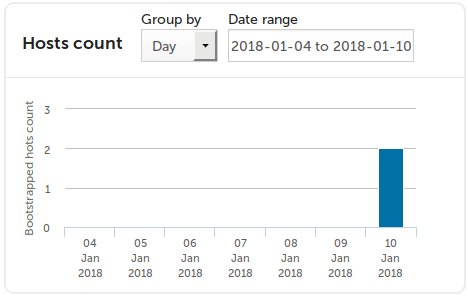
\includegraphics[width=.9\linewidth]{data/e9/0e4df9-0bb7-4a1e-84d5-25911497f93c/2018-01-10_Selection_001_2018-01-14_12-02-44.png}
\end{center}

\subsection*{mail settings}
\label{sec:org3486fbf}
\begin{itemize}
\item Exported reports can now be sent as attachments in emails
\end{itemize}

\begin{center}
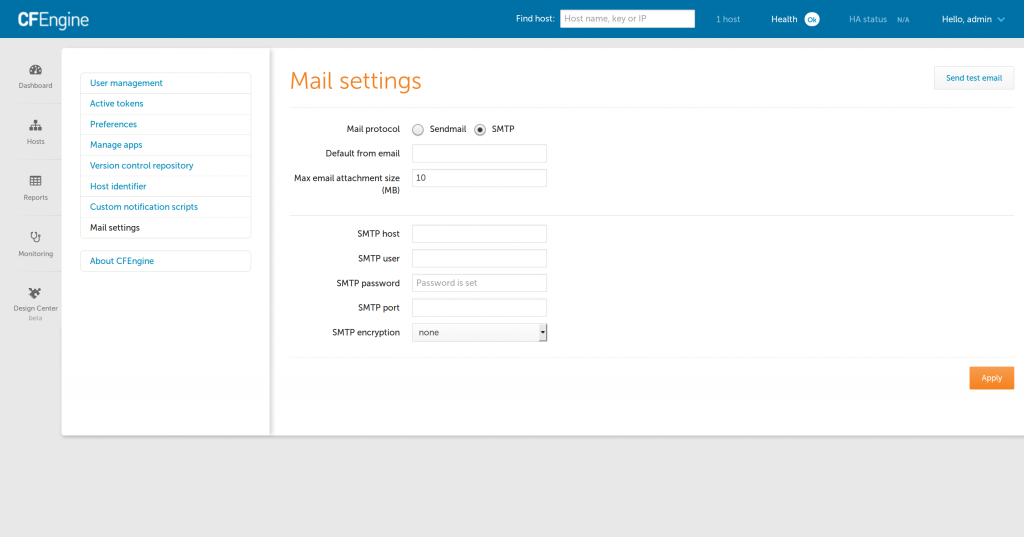
\includegraphics[width=.9\linewidth]{data/74/8d9e15-278e-46ac-822f-9e0f7e6b2830/mail-settings-1024x537_2018-01-14_12-01-05.png}
\end{center}

\subsection*{LDAP settings API}
\label{sec:orgaa99384}
\begin{center}
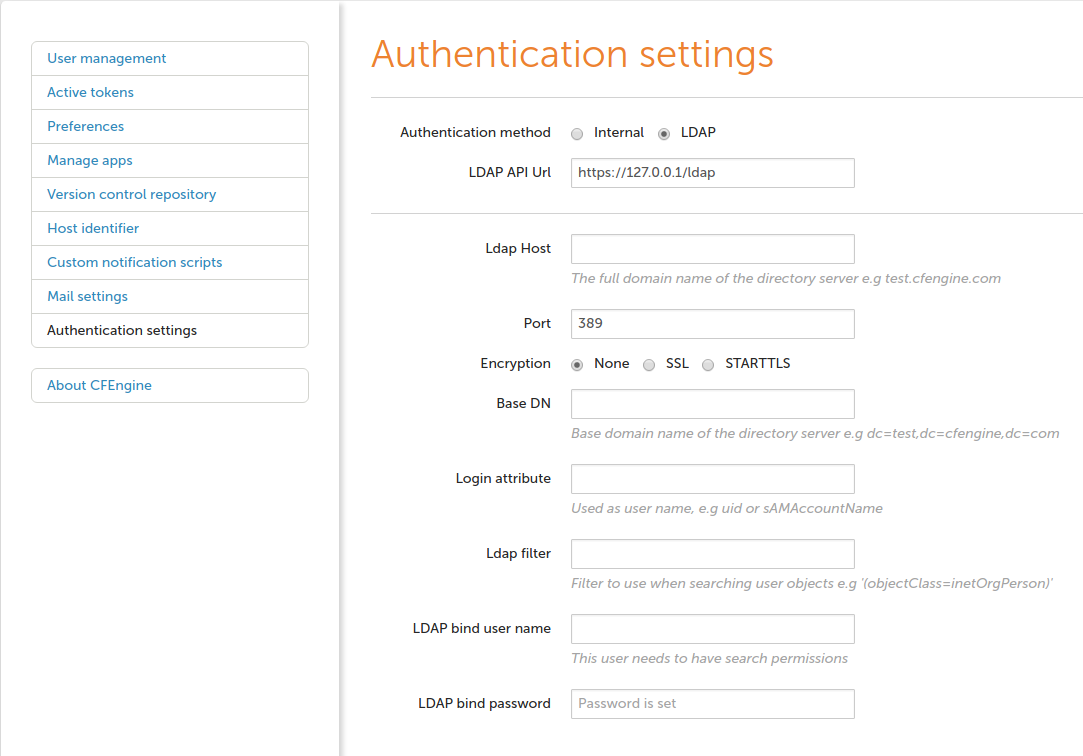
\includegraphics[width=.9\linewidth]{data/29/4c1258-49f4-4c72-9f8d-2b7535cfbea8/Authentication-settings_2018-01-14_12-04-18.png}
\end{center}

\subsection*{default roles}
\label{sec:org1d8ec8a}
\begin{center}
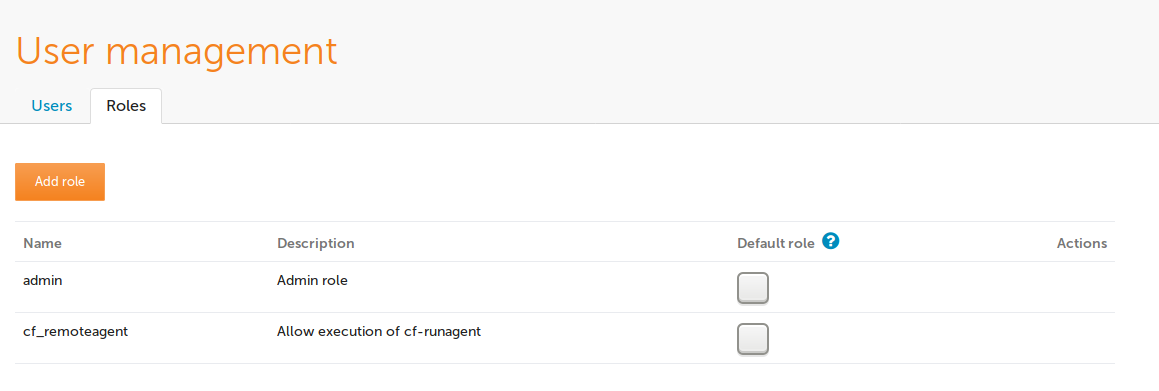
\includegraphics[width=.9\linewidth]{data/bf/10ec4b-5b6b-4140-9336-fb7ab7808fed/2018-01-14_Selection_004_2018-01-14_14-03-29.png}
\end{center}

\subsection*{New OOTB Inventory Attributes}
\label{sec:org4cfbb08}

\begin{itemize}
\item Policy Release Id
\item AIX OS Level
\end{itemize}

\subsection*{Inventory API}
\label{sec:org15c1182}

\begin{verbatim}
curl --user admin -X POST \
  -H 'content-type: application/json' \
  https://hub/api/inventory -d '{ "select":[ "Host name", "OS type"]}'
\end{verbatim}
\captionof{figure}{Example API Query}

\subsection*{Inventory API}
\label{sec:org120e0a8}

\begin{verbatim}
{
    "data": [
        {
            "header": [
                {
                    "columnName": "Host name",
                    "columnType": "STRING"
                },
                {
                    "columnName": "OS type",
                    "columnType": "STRING"
                }
            ],
            "queryTimeMs": 11,
            "rowCount": 2,
            "rows": [
                [
                    "host001",
                    "linux"
                ],
                [
                    "hub",
                    "linux"
                ]
            ]
        }
    ],
    "meta": {
        "count": 1,
        "page": 1,
        "timestamp": 1515607751,
        "total": 1
    }
}
\end{verbatim}
\captionof{figure}{Example Query Response}
\end{document}
